\documentclass[tikz,border=10pt,12pt]{standalone}
% Shared preamble for standalone-compiled dc_paper figures.
% Copies just the bits of dc_paper.tex's preamble that figures need.

\usepackage{amsmath,amssymb,amsthm,mathtools,bm}
\usepackage{siunitx}
\sisetup{detect-all,group-separator={,},per-mode=symbol}

\usepackage[T1]{fontenc}
\usepackage{xcolor}
\usepackage{enumitem}
\usepackage{mathpazo}                % Palatino body + matching math
\usepackage[scaled=0.92]{helvet}     % Helvetica sans
\usepackage{courier}                 % monospace
\usepackage{microtype}

% --- IA brand colour palette (must match dc_paper.tex) ---
\definecolor{iadark}{HTML}{1B1815}
\definecolor{iabone}{HTML}{FAFAF7}
\definecolor{iaaccent}{HTML}{A04A1F}
\definecolor{iataupe}{HTML}{F2EDE6}
\definecolor{iarule}{HTML}{3A332D}
\definecolor{iagrey}{HTML}{5A524A}

% --- graphics ---
\usepackage{tikz}
\usepackage{circuitikz}
\usepackage{pgfplots}
\pgfplotsset{compat=1.18}
\usetikzlibrary{arrows.meta,positioning,shapes.geometric,calc,fit,
                decorations.pathreplacing,decorations.markings,
                shadows.blur,backgrounds}

% --- math macros from dc_paper.tex preamble (figures use them) ---
\newcommand{\E}{\mathbb{E}}
\newcommand{\Var}{\operatorname{Var}}
\newcommand{\Cov}{\operatorname{Cov}}
\newcommand{\Cor}{\operatorname{Cor}}
\newcommand{\Prb}{\mathbb{P}}
\newcommand{\R}{\mathbb{R}}
\newcommand{\N}{\mathbb{N}}
\newcommand{\1}{\mathbf{1}}
\newcommand{\VaR}{\operatorname{VaR}}
\newcommand{\TVaR}{\operatorname{TVaR}}
\newcommand{\ES}{\operatorname{ES}}
\newcommand{\dd}{\mathrm{d}}
\newcommand{\given}{\,\vert\,}
\newcommand{\set}[1]{\left\{#1\right\}}
\newcommand{\norm}[1]{\left\Vert #1 \right\Vert}
\DeclareMathOperator*{\argmin}{arg\,min}
\DeclareMathOperator*{\argmax}{arg\,max}

% \textwidth has no meaning in standalone class; give it a value matching
% the paper's A4 + 1-inch margins so any leftover \resizebox{\textwidth}
% gracefully sizes the figure to that nominal width.
\setlength{\textwidth}{15.92cm}

\begin{document}
\pagecolor{iabone}
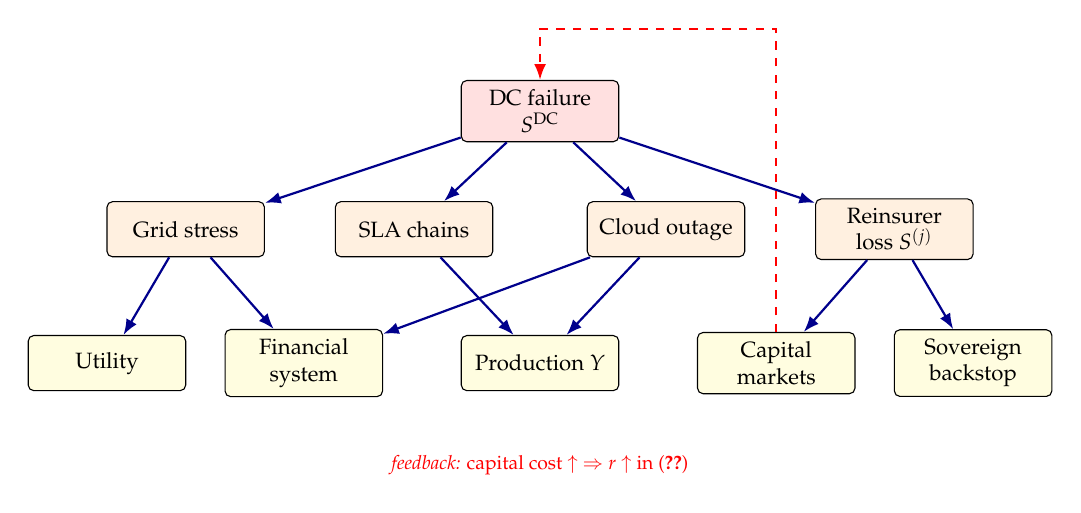
\begin{tikzpicture}[
   every node/.style={font=\footnotesize},
   sec/.style={draw,rectangle,rounded corners=2pt,minimum height=0.7cm,
               minimum width=2cm,align=center},
   primary/.style={sec,fill=red!12},
   secondary/.style={sec,fill=orange!12},
   tertiary/.style={sec,fill=yellow!12},
   recovery/.style={sec,fill=green!12},
   arr/.style={-{Latex[length=2mm]},thick,blue!55!black}
]
% Layer 1
\node[primary] (DC) at (0,4) {DC failure\\$S^{\mathrm{DC}}$};

% Layer 2: direct propagations
\node[secondary] (GR) at (-4.5,2.5) {Grid stress};
\node[secondary] (SLA) at (-1.6,2.5) {SLA chains};
\node[secondary] (CL) at (1.6,2.5) {Cloud outage};
\node[secondary] (RS) at (4.5,2.5) {Reinsurer\\loss $S^{(j)}$};

\draw[arr] (DC) -- (GR);
\draw[arr] (DC) -- (SLA);
\draw[arr] (DC) -- (CL);
\draw[arr] (DC) -- (RS);

% Layer 3: real-economy
\node[tertiary] (UT) at (-5.5,0.8) {Utility};
\node[tertiary] (FIN) at (-3,0.8) {Financial\\system};
\node[tertiary] (PROD) at (0,0.8) {Production $Y$};
\node[tertiary] (CAP) at (3,0.8) {Capital\\markets};
\node[tertiary] (SOV) at (5.5,0.8) {Sovereign\\backstop};

\draw[arr] (GR) -- (UT);
\draw[arr] (GR) -- (FIN);
\draw[arr] (SLA) -- (PROD);
\draw[arr] (CL) -- (PROD);
\draw[arr] (CL) -- (FIN);
\draw[arr] (RS) -- (CAP);
\draw[arr] (RS) -- (SOV);

% Feedback to DC: routed OVER the top of the diagram through the clean
% vertical channel between Cloud outage (x in [0.6,2.6]) and Reinsurer
% (x in [3.5,5.5]). Crosses no boxes, and frees the bottom strip for the
% explanatory label.
\draw[arr,dashed,red]
   (CAP.north) -- ++(0,3.85)            % up at x=3, between CL and RS
   -- ++(-3,0)                          % left across the top at y=5
   -- (DC.north);                       % down into DC top
\node[red,font=\scriptsize,align=center,anchor=north] at (0,-0.25)
   {\textit{feedback:} capital cost $\uparrow$ $\Rightarrow$ $r$ $\uparrow$
    in \eqref{eq:opercost}};

\end{tikzpicture}
\end{document}
